\documentclass{uebblatt}

\begin{document}

\maketitle{2}{-- \emph{Spiel und Spaß mit Verklebedaten} --}

\begin{aufgabe}{Geometrische Realiserung des simplizialen
Standard-$p$-Simplexes}
Wir wollen an einem Beispiel nachvollziehen, dass die Grundlagen
der Theorie der simplizialen Mengen sinnvoll aufeinander abgestimmt sind:
Zeige, dass die geometrische Realisierung~$|\Delta[p]|$ des simplizialen
Standard-$p$-Simplex kanonisch homöomorph zum topologischen
Standard-$p$-Simplex~$\Delta_p$ ist.

Gib dazu explizit die kanonische Abbildung~$|\Delta[p]| \to \Delta_p$ an und
weise nach, dass sie ein Homöomorphismus ist. Später werden wir lernen, wie man
diese Aufgabe auch unmittelbar vermöge abstrakten Nonsens lösen kann.
\end{aufgabe}

\begin{aufgabe}{Simpliziale Mengen aus Verklebedaten}
In der Vorlesung wurde eine Konstruktion beschrieben, um aus einem
Verklebedatum~$(X_{(n)})$ eine simpliziale Menge~$\widetilde X$ zu bauen: Als
Menge der~$m$-Simplizes nimmt man dabei
\[ \widetilde X_m := \coprod_{\substack{k \geq 0 \\ g : [m] \twoheadrightarrow [k]}} X_{(k)}, \]
Ein~$m$-Simplex von~$\widetilde X$ ist also ein Tupel~$(g,x)$, wobei~$g : [m]
\to [k]$ eine monotone Surjektion (mit~$k \geq 0$ beliebig) und~$x \in X_{(k)}$
ein~$k$-Simplex von~$X$ ist; wir stellen es uns als "`Degeneration von~$x$
längs~$g$"' vor. (Wenn~$g$ die Identität ist, ist das keine gute Vorstellung --
sonst aber schon.)

Ist~$f : [n] \to [m]$ eine monotone Abbildung, so definiert
man~$\widetilde X(f)(g,x) := (\pi, X(\iota)x)$, wobei~$[n]
\xrightarrow{\pi} [\ell] \xrightarrow{\iota} [k]$ die eindeutige Epi/Mono-Zerlegung
von~$g \circ f$ ist.
\begin{enumerate}
\item Zeige, dass diese Setzung wirklich zu einer simplizialen Menge führt,
weise also die beiden Axiome über~$\widetilde X$ nach.
\item Zeige, dass~$\widetilde X$ folgende besondere Eigenschaft hat: Für jedes
nichtdegenerierte Simplex~$x \in \widetilde X_m$ und jede monotone Injektion~$f
: [n] \to [m]$ ist das Simplex~$\widetilde X(f)x \in \widetilde X_n$
ebenfalls nichtdegeneriert.

\emph{Tipp:} Vielleicht hilft es dir, nachzuweisen, dass ein Simplex~$(g,x) \in
\widetilde X_m$ genau dann nichtdegeneriert ist, wenn~$g$ eine
Identitätsabbildung ist.

\item Zeige, dass eine beliebige simpliziale Menge genau dann durch die
beschriebene Konstruktion von einem Verklebedatum stammt, wenn es die
Eigenschaft aus Teilaufgabe~b) hat.
\end{enumerate}

Die Konstruktion~$X \mapsto \widetilde X$ stellt einen Linksadjungierten zum
Vergissfunktor von der Kategorie der simplizialen Mengen in die Kategorie der
Verklebedaten dar. In einem gewissen Sinn kann man sie als Kategorifizierung
des Fundamentalsatzes von Newtons Finite-Differenzen-Kalkül ansehen.
Siehst du eine Verbindung?
\[ a_m = \sum_{k=0}^m \binom{m}{k} (\partial^k a)_0. \]
\end{aufgabe}

\vspace{-\aufgabenskip}

\begin{aufgabe}{Basiswissen zu Homotopie}
Ein topologischer Raum~$X$ heißt genau dann \emph{zusammenziehbar}, wenn es
einen Basispunkt~$x_0 \in X$ derart gibt, dass eine stetige Abbildung~$H :
X \times [0,1] \to X$ mit~$H(x,0) = x$ und~$H(x,1) = x_0$ für alle~$x \in X$
existiert.

Eine stetige Abbildung~$f : X \to Y$ heißt genau dann
\emph{Homotopieäquivalenz}, wenn es eine stetige Abbildung~$g : Y \to X$ derart
gibt, dass~$g \circ f$ und~$f \circ g$ (zwar nicht unbedingt gleich, aber)
homotop zur jeweiligen Identitätsabbildung sind. Zwei Räume heißen genau dann
zueinander \emph{homotopieäquivalent}, wenn eine Homotopieäquivalenz
zwischen ihnen verläuft.

Beweise so viele der folgenden Behauptungen, wie du möchtest.

\begin{enumerate}
\item Ein Raum ist genau dann zusammenziehbar, wenn er homotopieäquivalent zu
einem einpunktigen Raum ist.
\item Ist~$X$ zusammenziehbar, so sind je zwei stetige Abbildungen~$Y
\rightrightarrows X$ zueinander homotop. Die Umkehrung gilt ebenfalls. (Das
Konzept von Homotopie von Abbildungen kann man sich also nicht gut anhand von
Abbildungen~$\RR \to \RR$ veranschaulichen.)
\item Zusammenziehbare Räume sind stets wegzusammenhängend.
\item \hcancel{Der leere Raum ist zusammenziehbar.}{0pt}{3pt}{0pt}{-2pt}
\end{enumerate}
\end{aufgabe}

\end{document}

\begin{aufgabe}{Fasernde simpliziale Mengen}
Eine simpliziale Menge~$X$ heißt genau dann \emph{fasernd}, wenn für jedes~$n
\geq 0$ und~$k$ mit~$0 \leq k \leq n + 1$ folgende Bedingung erfüllt ist:
\begin{quote}Sind Simplizes~$x_0,\ldots,x_{k-1},x_{k+1},\ldots,x_{n+1} \in X_n$
mit~$d_i x_j = d_{j-1} x_i$ für alle~$i < j$ (wobei~$i$ und~$j$ ungleich~$k$)
vorgegeben, so existiert ein Simplex~$y \in X_{n+1}$ mit~$d_i(y) = x_i$ für
alle~$i \neq k$.
\end{quote}
\begin{enumerate}
\item Was bedeutet diese Bedingung anschaulich? Denke dazu an \emph{Hörner}.
\begin{center}
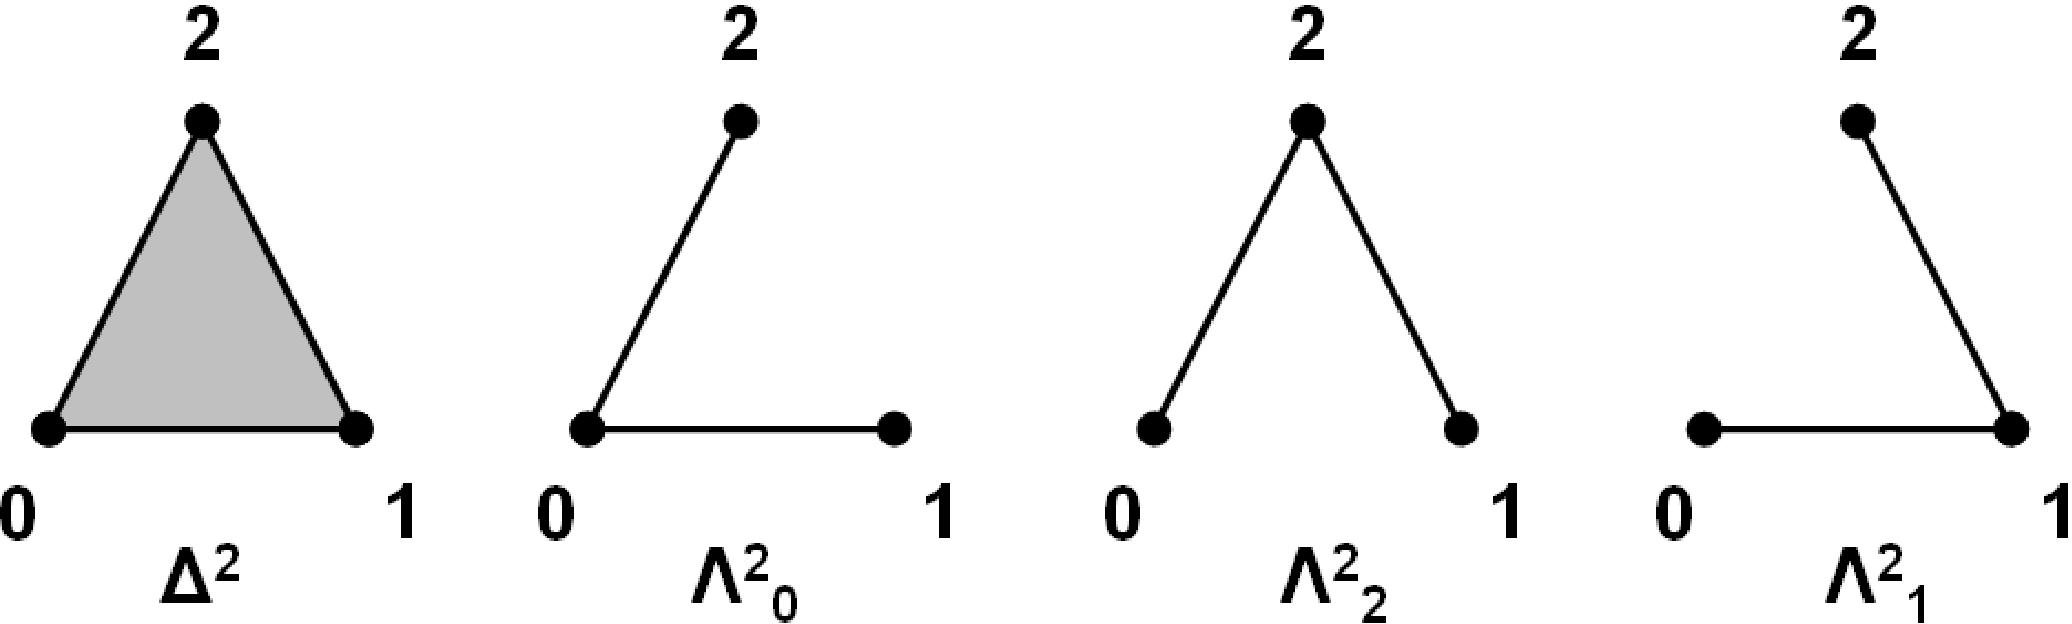
\includegraphics[scale=0.5]{hoerner}

Abbildung: Die drei Hörner von~$\Delta^2$.
\end{center}
\end{enumerate}
\end{aufgabe}
